\documentclass[12pt]{article}

\usepackage{amsfonts}
\usepackage{svg}
\usepackage{setspace}
\usepackage{caption}
\usepackage{subcaption}
\usepackage{float}
\usepackage{makecell}
\usepackage{amsmath}
\usepackage{graphicx}
\graphicspath{ {./images/} }
\usepackage[utf8]{inputenc}
\usepackage[russian]{babel}
\usepackage{geometry}
 \geometry{
 a4paper,
 left=20mm,
 right=20mm,
 top=20mm,
 bot=20mm,
 }

\begin{document}

\begin{titlepage}
\begin{center}
    {\small НАЦИОНАЛЬНЫЙ ИССЛЕДОВАТЕЛЬСКИЙ УНИВЕРСИТЕТ ИТМО} \\
    {\small Факультет систем управления и робототехники} \\
    \vspace*{10\baselineskip}

    \begin{spacing}{1.2}
    {\LARGE ТЕОРИЯ АВТОМАТИЧЕСКОГО УПРАВЛЕНИЯ \\
    Лабораторная работа №4 \\
    Удержание заданного положения надводного судна\\}
    \end{spacing}
    \ \\
    \vspace*{10\baselineskip}
    \hfill {\small Выполнил студент:} \\
    \hfill {\small Кирбаба Д.Д. R3338} \\
    \ \\
    \hfill {\small Преподаватель:} \\
    \hfill {\small Бобцов А.А.} \\
    \mbox{}
    \vfill {\smallг. Санкт-Петербург\\2023}
\end{center}
\end{titlepage}

\section*{Цель работы}
Стабилизация положения надводного судна с помощью трех регуляторов:
\begin{itemize}
  \item ПИД;
  \item Последовательный компенсатор;
  \item Регулятор на основе наблюдателя с высоким коэффициентом усиления (High-gain).
\end{itemize}

\section*{Постановка задачи}
Рассмотрим линеаризованную модель надводного судна
\[
M \ddot{y} + D \dot{y} = \tau +\tau_d,
\]
где $y = \begin{bmatrix} X & Y & \Phi \end{bmatrix} ^T$ - вектор координат надводного судна относительно параллельной системы координат, связанной с судном,
\[
M = \begin{bmatrix}
    3 & 0 & 0 \\
    0 & 3 & -0.5 \\
    0 & -0.5 & 1 \\
\end{bmatrix}, \
D = \begin{bmatrix}
    1 & 0 & 0 \\
    0 & 1 & 1 \\
    0 & 1 & 1 \\
\end{bmatrix}, \
\tau_d = \begin{bmatrix} \tau_{d1} \\ \tau_{d2} \\ \tau_{d3} \end{bmatrix} =
\begin{bmatrix} 1 \\ 2 \\ 3 \end{bmatrix}.
\]
\begin{figure}[H]
    \centering
    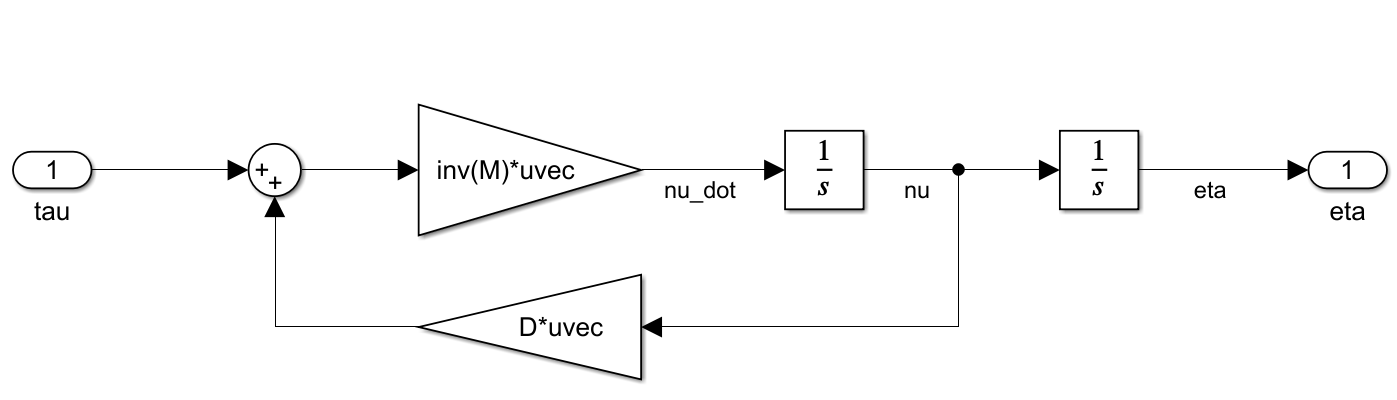
\includegraphics[width=0.7\textwidth]{model.png}
    \caption{Линеаризованная модель.}
    \label{fig:model.png}
\end{figure}\\
Выполним моделирование задачи удержания заданного положения в базовой системе координат
\[
y^b_r = \begin{bmatrix} X^b_r \\ Y^b_r \\ \Phi^b_r \end{bmatrix},
\] которое на каждом такте преобразуется в систему координат, связанную с судном с помощью
\[
y_r = \begin{bmatrix}
    \cos{\Phi} & \sin{\Phi} & 0 \\
    -\sin{\Phi} & \cos{\Phi} & 0 \\
    0 & 0 & 1 \\
\end{bmatrix}.
\]
Необходимо синтезировать закон управления обеспечивающий выполнение целевого условия для
сколь угодно малого $\epsilon > 0$
\[
\lim_{t \rightarrow \infty} \norm{\tilde{y}} \leq \epsilon,
\]
где $\tilde{y} = y(t) - y_r(t)$ — ошибка между выходом объекта $y(t)$ и референсной траекторией, которая в данном случае задается точкой $y_r(t) = y_r$. Точка $y_r$ для моделирования может быть назначена произвольным образом, однако, стоит обратить внимание, что в дальнейшей экспериментальной апробации точка должна находиться в пределах рабочей области бассейна, которая составляет $[1920 \times 840]$px, при этом предпочтительнее располагать ее ближе к центральной области.

\begin{figure}[H]
    \centering
    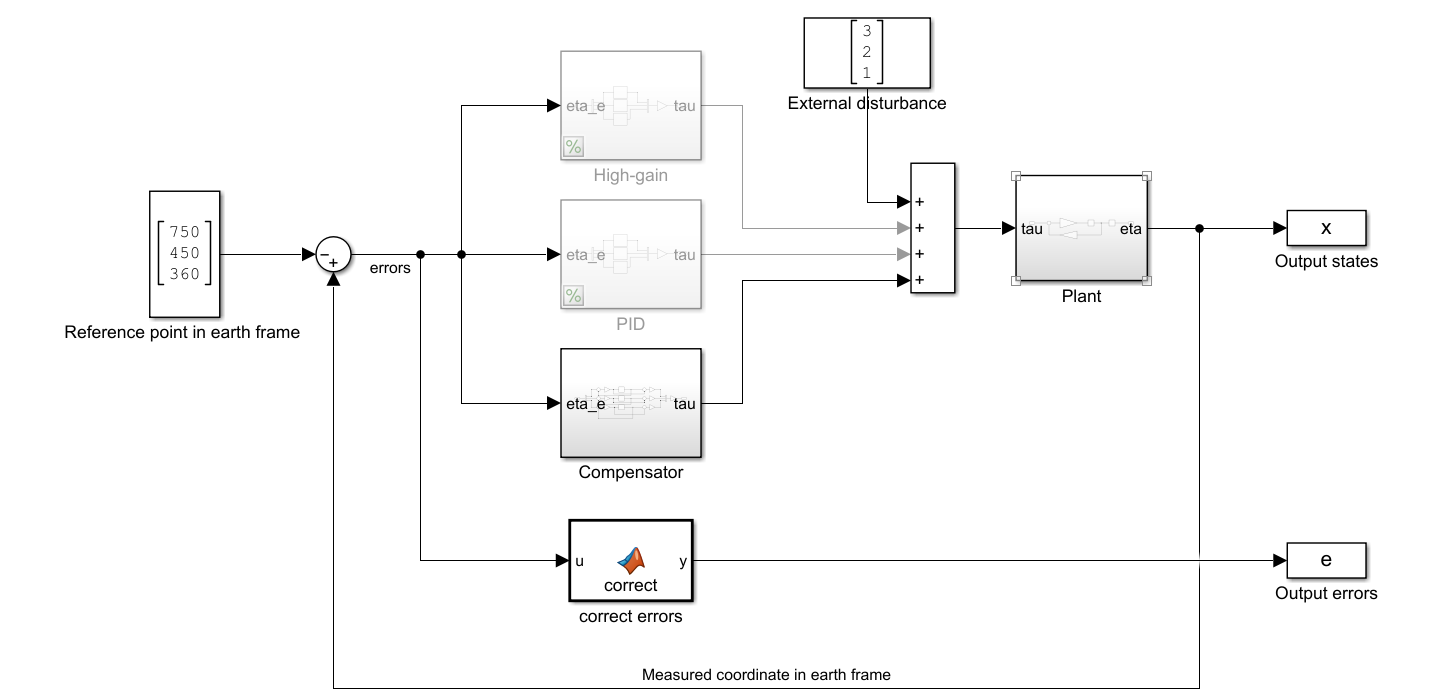
\includegraphics[width=\textwidth]{lin_model_scheme.png}
    \caption{Блок-схема линейной модели судна.}
    \label{fig:lin_model_scheme.png}
\end{figure}\\

\section*{ПИД-регулятор}
Пропорционально-интегрально-дифференциальный регулятор - это механизм управления, использующий обратную связь.\\
Математическая форма:
\[
u(t) = K_p e(t) + K_i \int_{0}^{t} e(\tau) \, d\tau + K_d \frac{de(t)}{dt}.
\]
\begin{figure}[H]
    \centering
    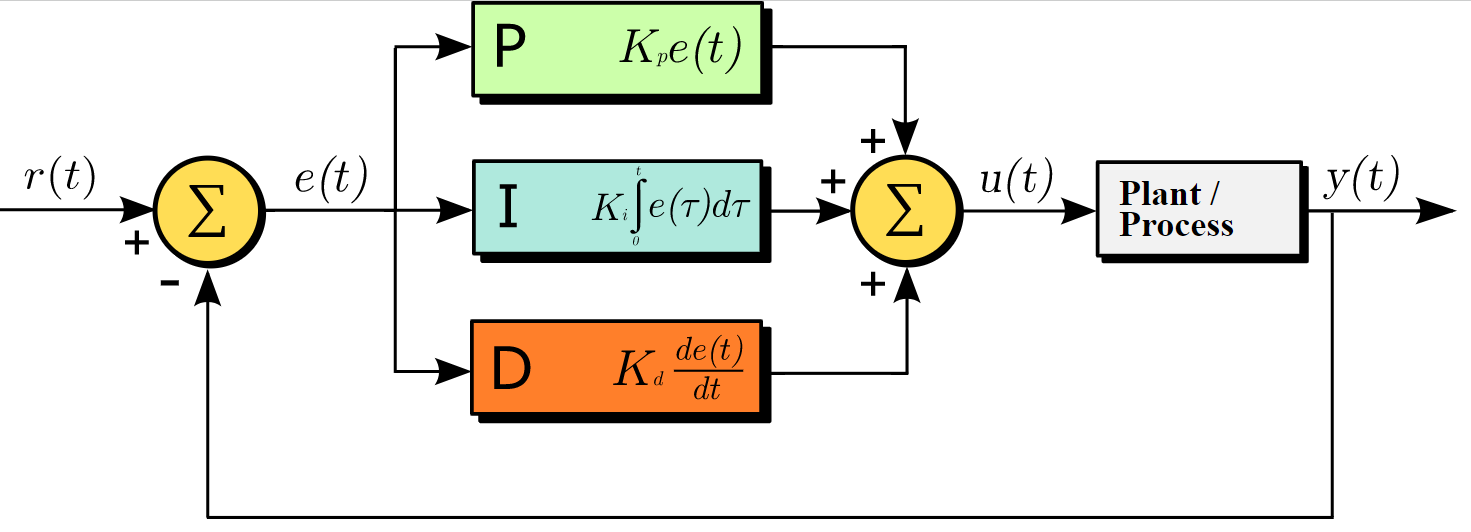
\includegraphics[width=0.7\textwidth]{PID_scheme.png}
    \caption{Блок-схема ПИД-регулятора.}
    \label{fig:PID_scheme.png}
\end{figure}\\

Встроим ПИД-регулятор для всех трех компонент вектора состояний судна.
\begin{figure}[H]
    \centering
    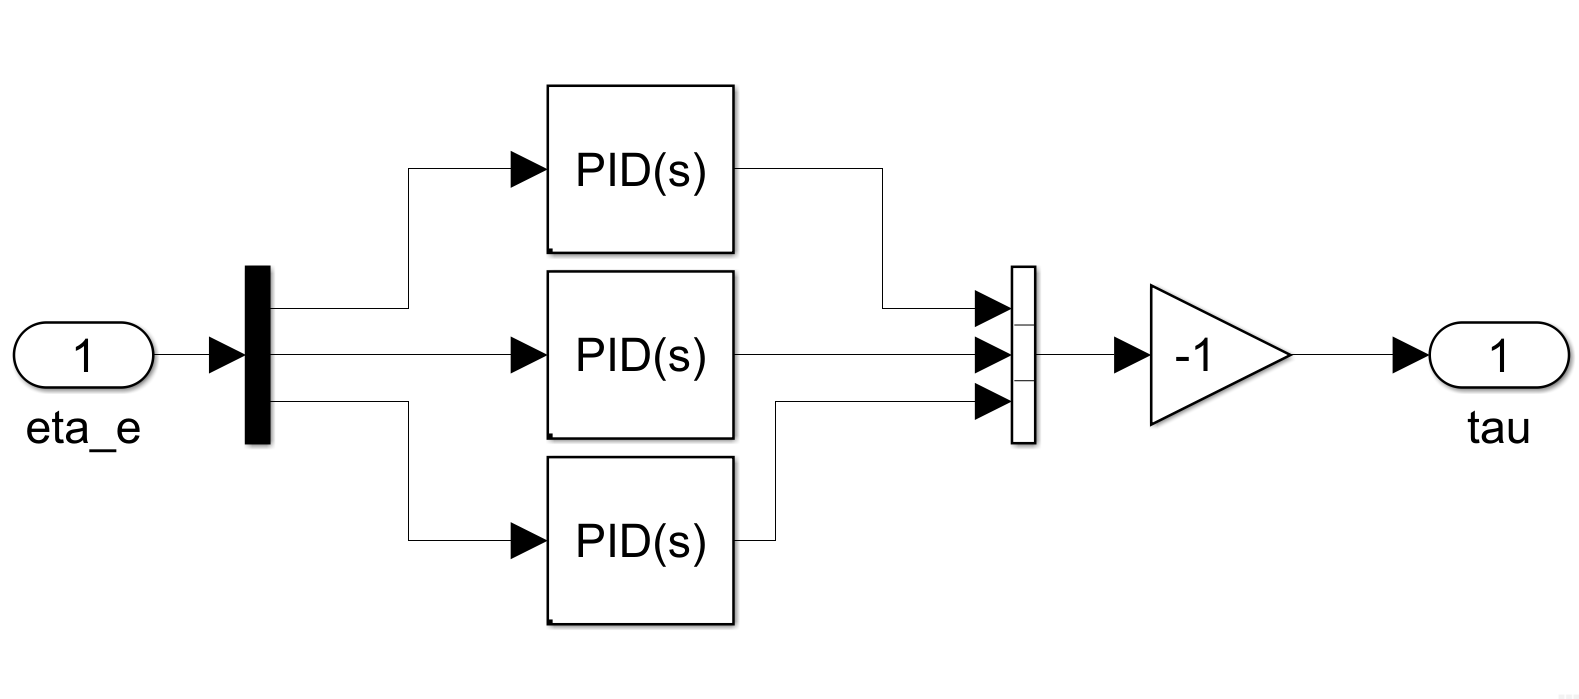
\includegraphics[width=0.7\textwidth]{pid_simulink_scheme.png}
    \caption{Схема ПИД-регулятора для каждого компонента вектора состояний.}
    \label{fig:pid_simulink_scheme.png}
\end{figure}\\
\ \\
Итого, необходимо подобрать 9 коэффициентов. \\
Подобранные коэффициенты:
\[ K = 
\begin{bmatrix}
    30 & 20 & 200 \\
    1 & 1 & 1 \\
    100 & 100 & 100 \\
\end{bmatrix}
\]
Цель управления: $y_{goal} = \begin{bmatrix}
    750 \\ 450 \\ 0
\end{bmatrix}.$
Начальное положение: $y_{initial} = \begin{bmatrix}
    559 \\ 517 \\ 301
\end{bmatrix}.$
\ \\
Приведем графики эксперимента и моделирования:
\begin{figure}[H]
    \centering
    \begin{subfigure}{0.49\textwidth}
        \centering
        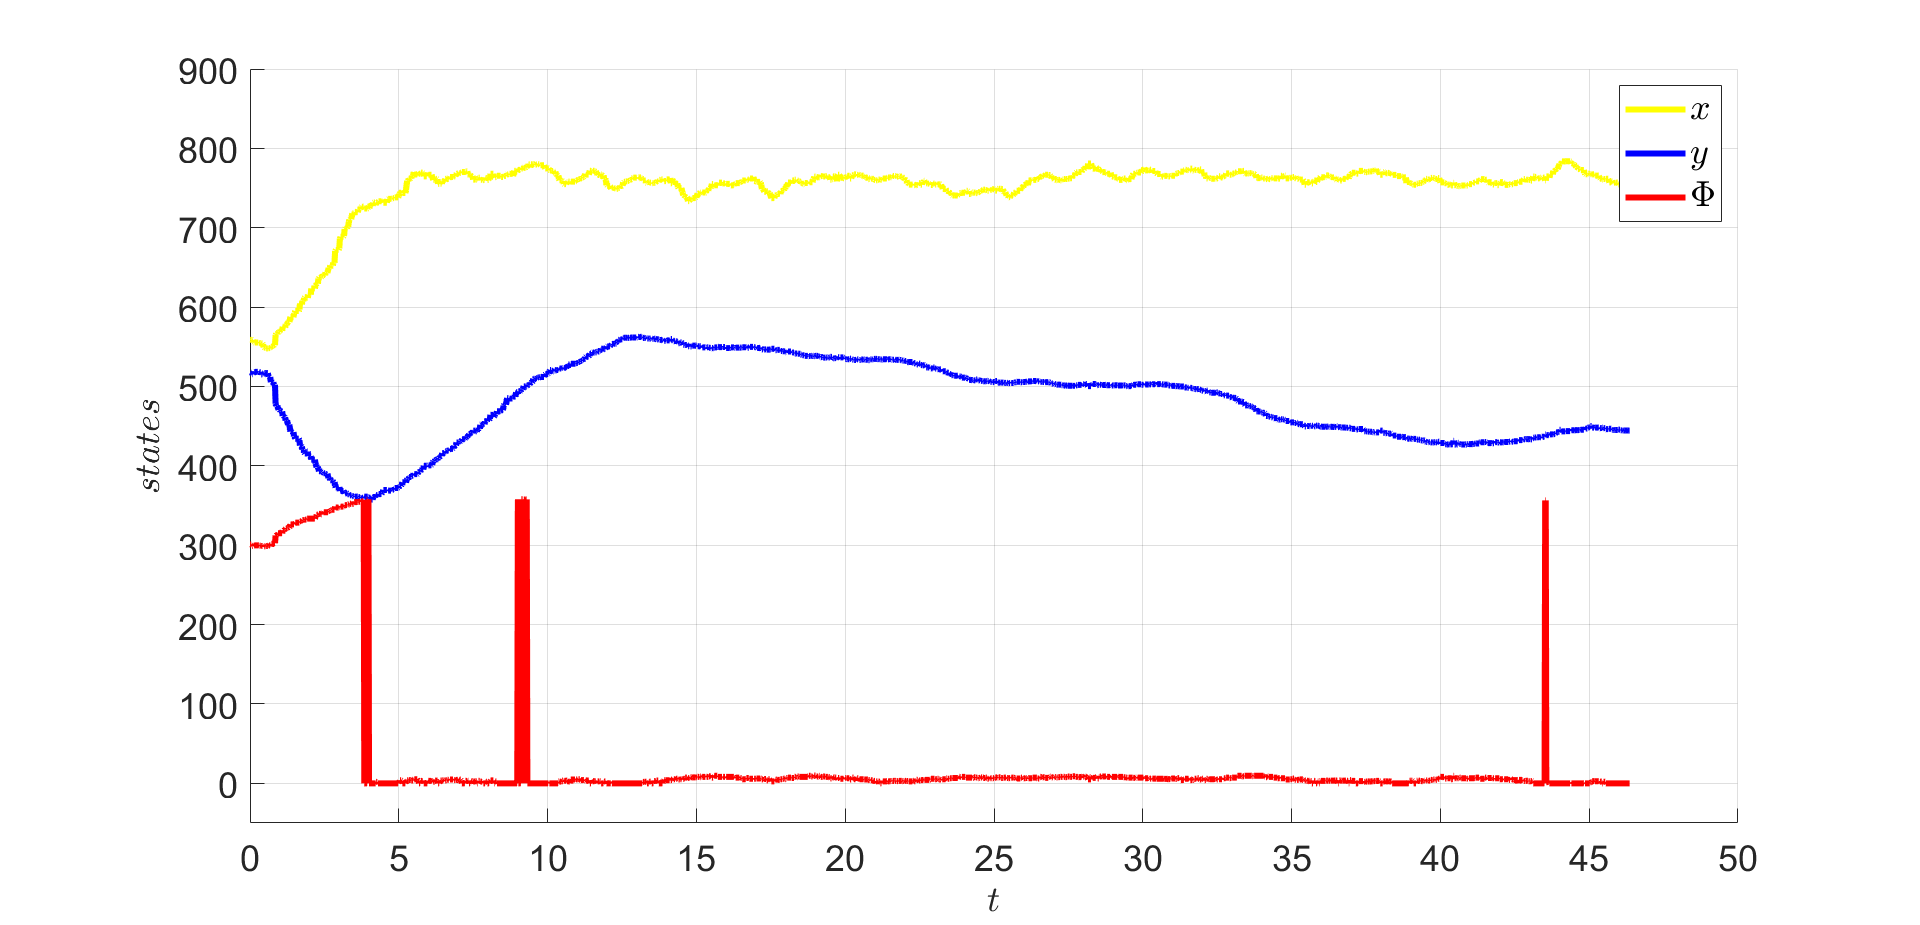
\includegraphics[width=\textwidth]{pid_x.png}
        \caption{эксперимент}
         \label{fig:pid_x.png}
     \end{subfigure}
     \hfill
     \begin{subfigure}{0.49\textwidth}
         \centering
         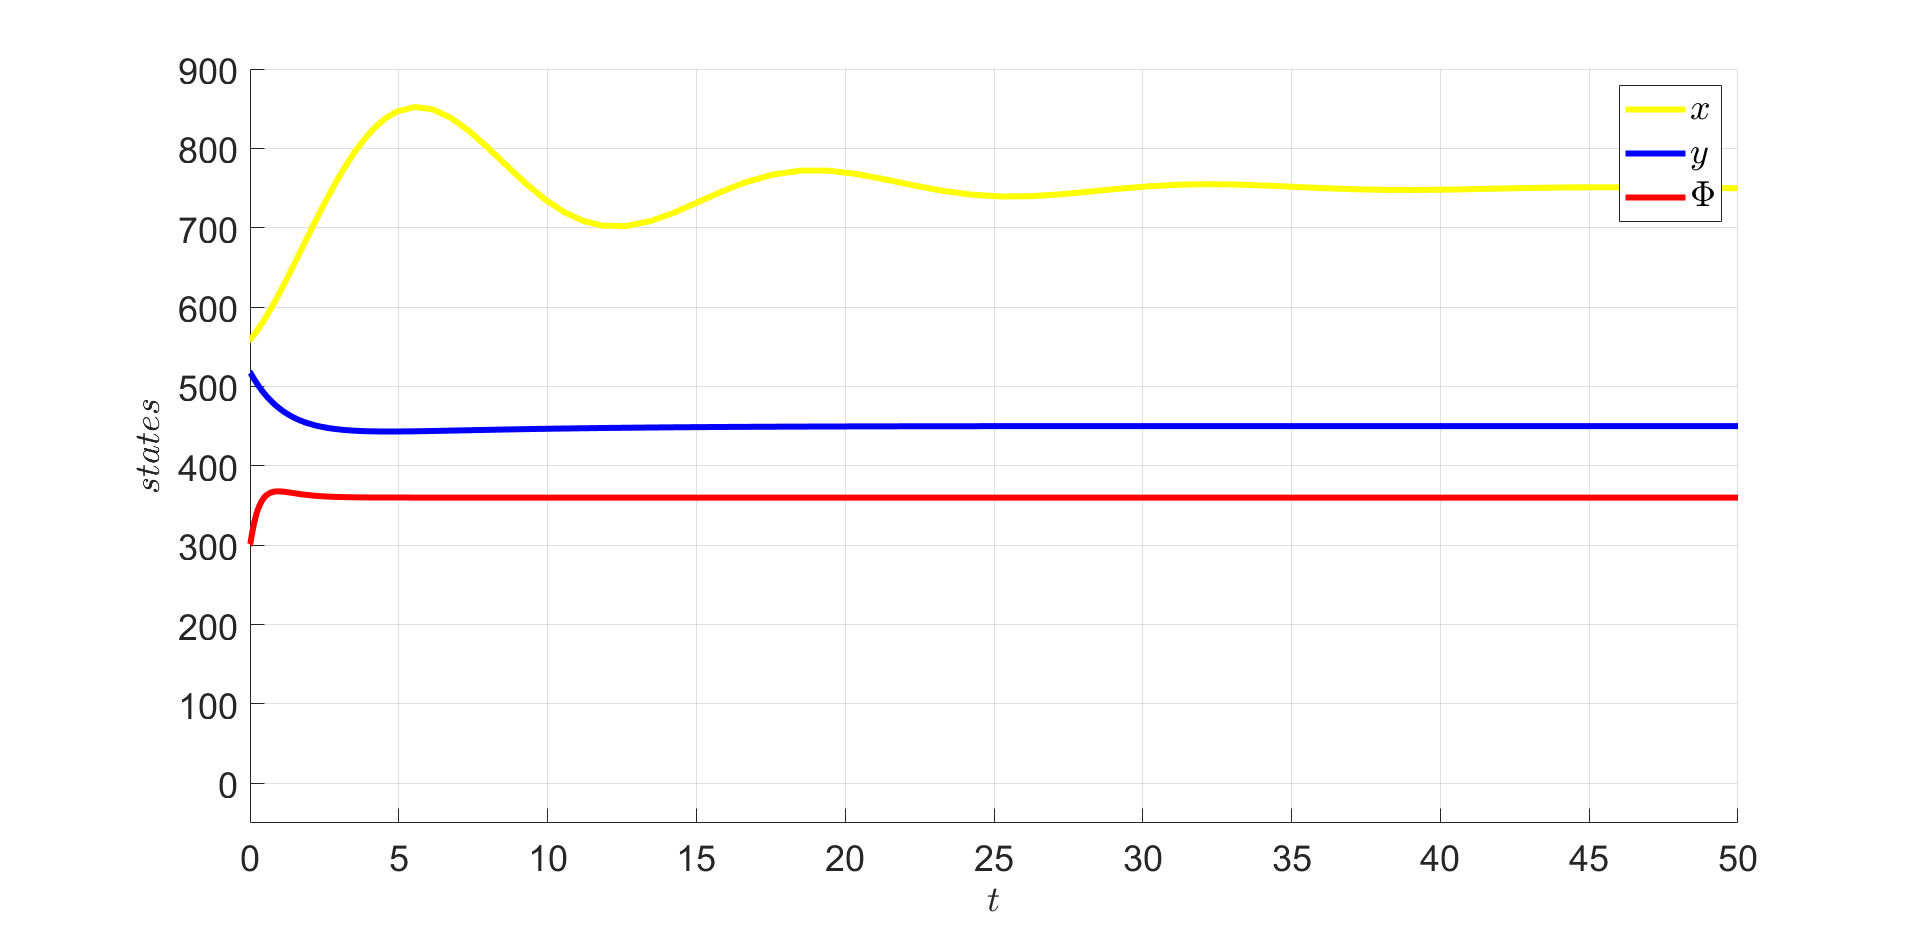
\includegraphics[width=\textwidth]{pid_x_modeling.png}
         \caption{моделирование}
         \label{fig:pid_x_modeling.png}
     \end{subfigure}
    \caption{Графики переходных процессов.}
    \label{fig:two graphs}
\end{figure}

\begin{figure}[H]
    \centering
    \begin{subfigure}{0.49\textwidth}
        \centering
        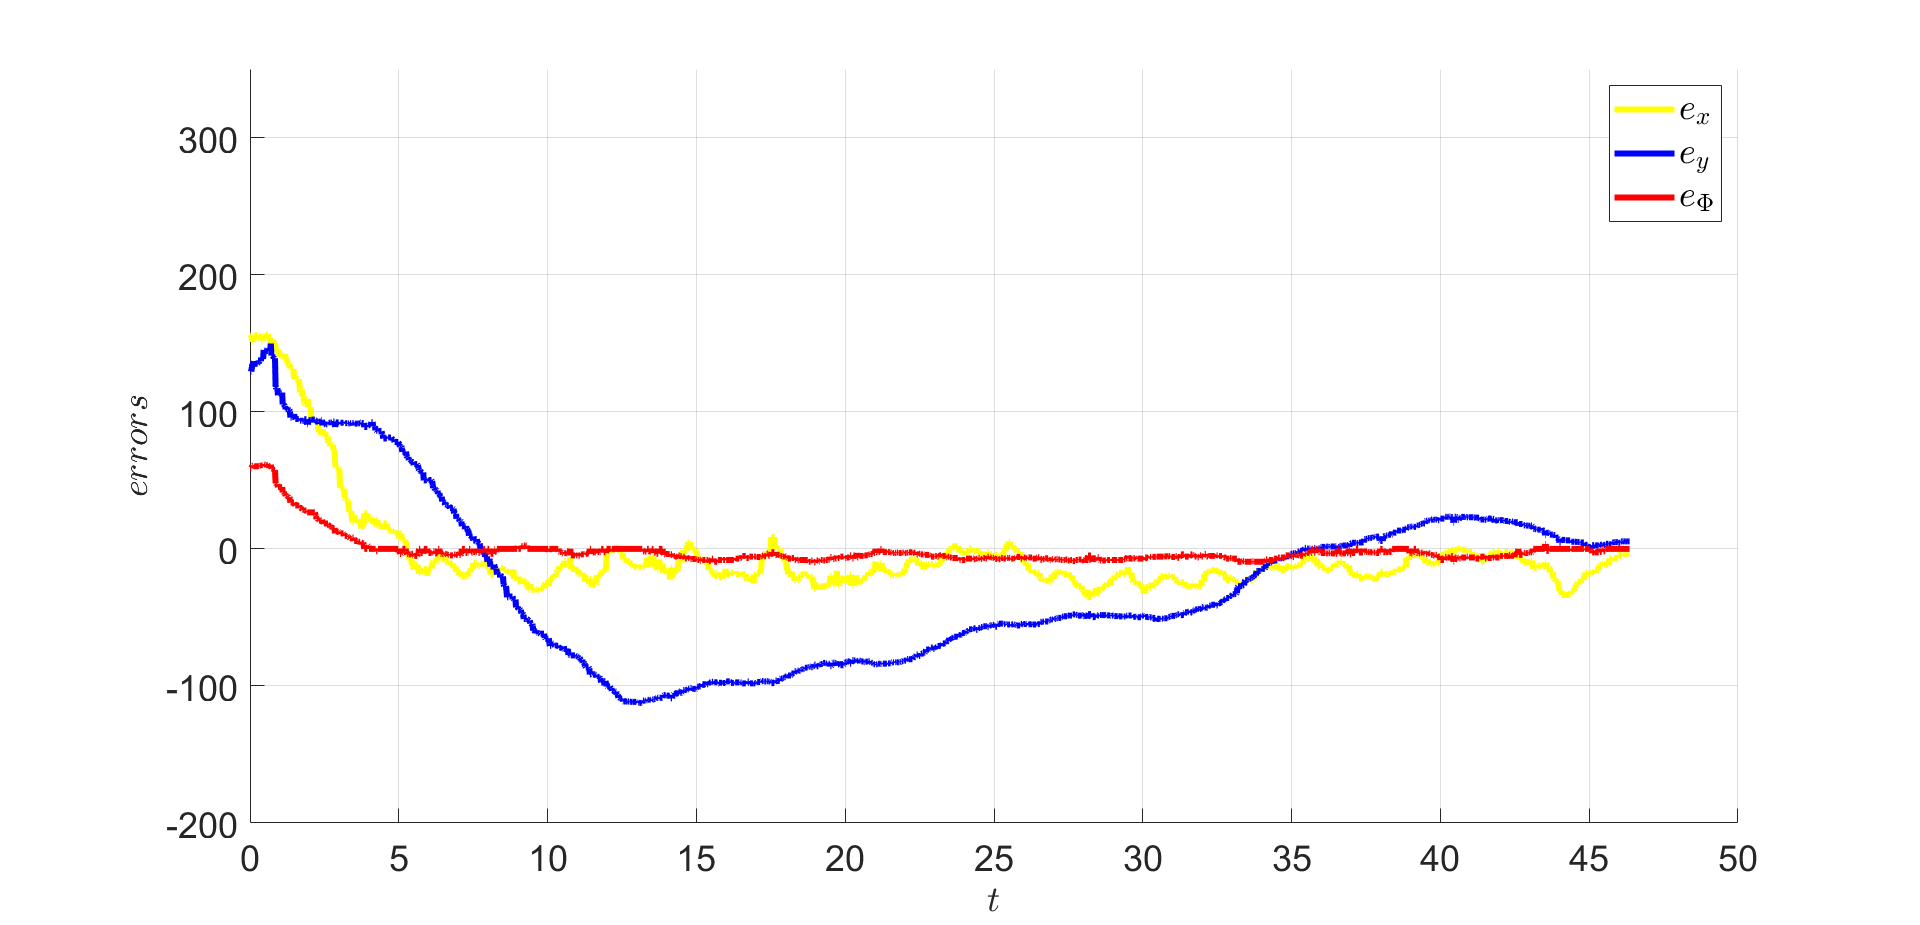
\includegraphics[width=\textwidth]{pid_e.png}
        \caption{эксперимент}
         \label{fig:pid_e.png}
     \end{subfigure}
     \hfill
     \begin{subfigure}{0.49\textwidth}
         \centering
         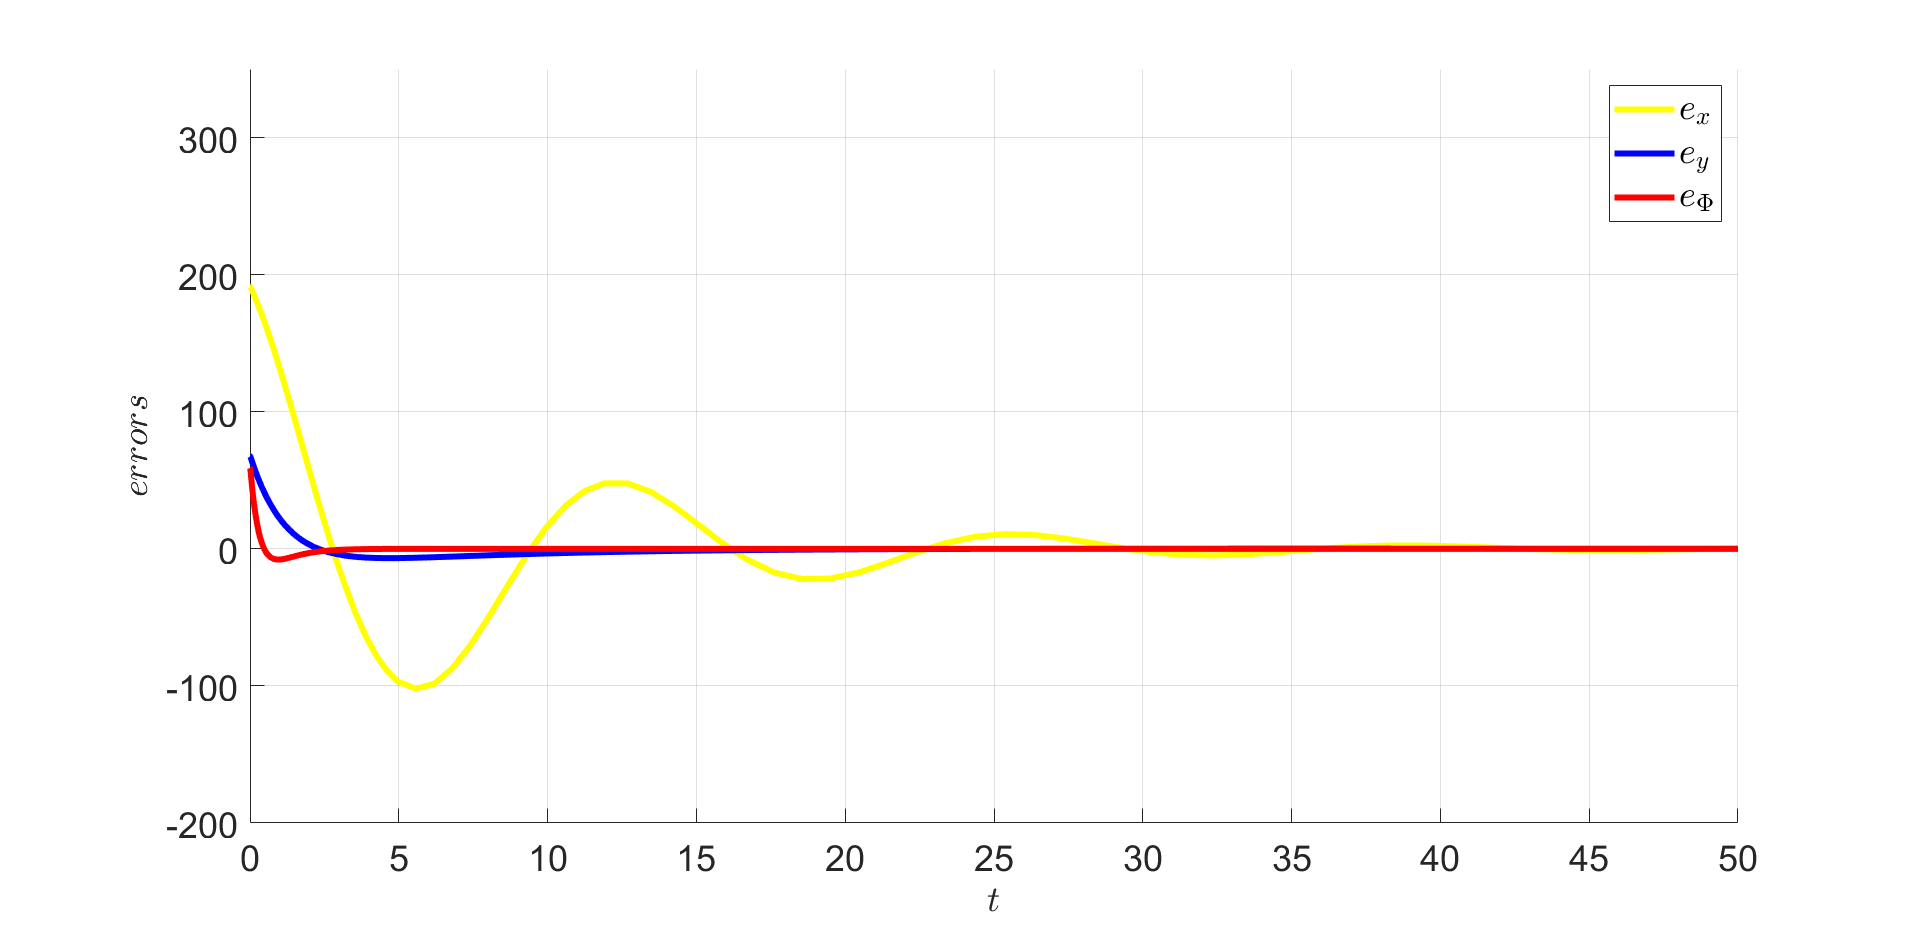
\includegraphics[width=\textwidth]{pid_e_modeling.png}
         \caption{моделирование}
         \label{fig:pid_e_modeling.png}
     \end{subfigure}
    \caption{Графики ошибок.}
    \label{fig:two graphs}
\end{figure}

ПИД-регулятор смог стабилизировать систему, однако время переходного процесса составило около 40 секунд при эксперименте. Преимуществом данного метода является простота математического аппарата.\\
Также подбор коэффициентов не являлся сложным из-за их понятной интерпретации ($K_p$ - обычная пропорциональная составляющая ошибки, $K_i$ - учитывает прошлые значения ошибок и накапливает их с течением времени, $K_d$ - оценка будущего тренда ошибки, основанная на текущем темпе её изменения).

\section*{Последовательный компенсатор}
Выберем закон управления на основе метода последовательного компенсатора:
\[
\begin{cases}
    u(t) = \mu_i(\dot{\xi_i} + \xi_i) \\
    \dot{\xi_i} = \sigma_i(-\xi_i + e_i), \\
\end{cases}
\]
где $\mu_i, \ \sigma_i, \ i = x, \ y, \ \varphi$ настраиваемые коэффициенты регулятора.\\
\ \\
Выбранные параметры:
\[
\sigma = \begin{bmatrix}
    10 \\ 10 \\ 10 \\
\end{bmatrix}, \ \mu = \begin{bmatrix}
    100 \\ 200 \\ 300 \\
\end{bmatrix}
\]

\begin{figure}[H]
    \centering
    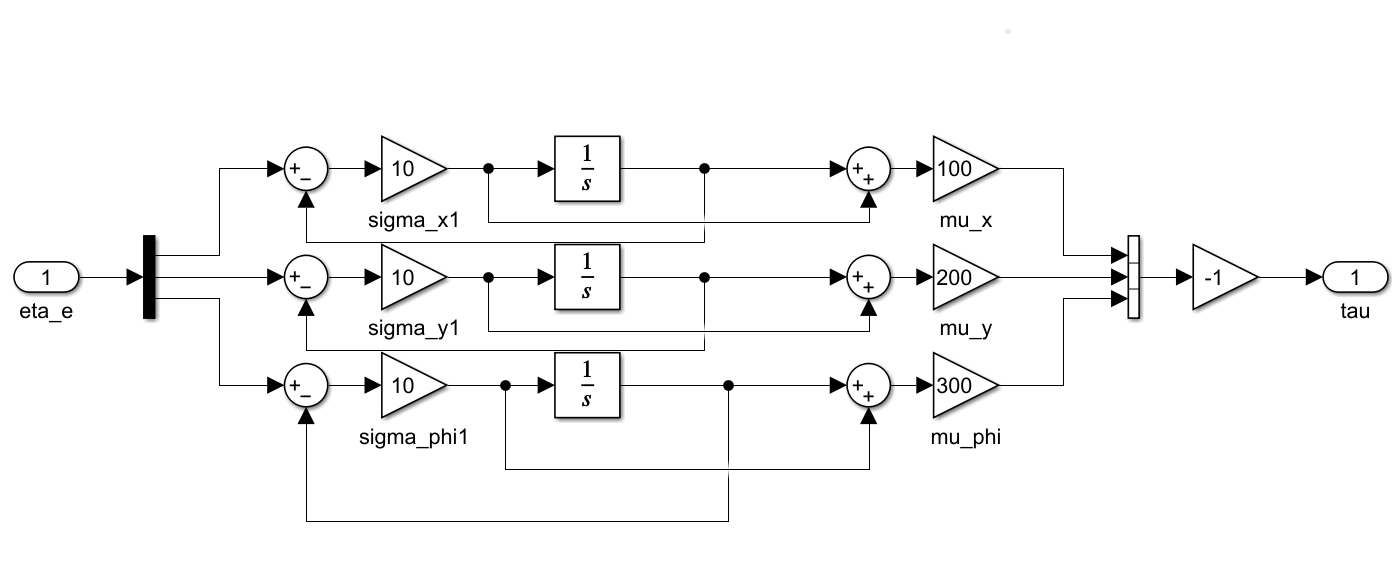
\includegraphics[width=0.7\textwidth]{compensator_scheme.png}
    \caption{Последовательный компенсатор.}
    \label{fig:compensator_scheme.png}
\end{figure}\\

Эксперимент с последовательным компенсатором был проведен при следующем начальном условии:
\[
y_{initial} = \begin{bmatrix}
    559 \\ 517 \\ 301
\end{bmatrix}.
\]
Референская точка:
\[
y_{goal} = \begin{bmatrix}
    750 \\ 450 \\ 0
\end{bmatrix}
\]
Приведем графики эксперимента и моделирования:
\begin{figure}[H]
    \centering
    \begin{subfigure}{0.49\textwidth}
        \centering
        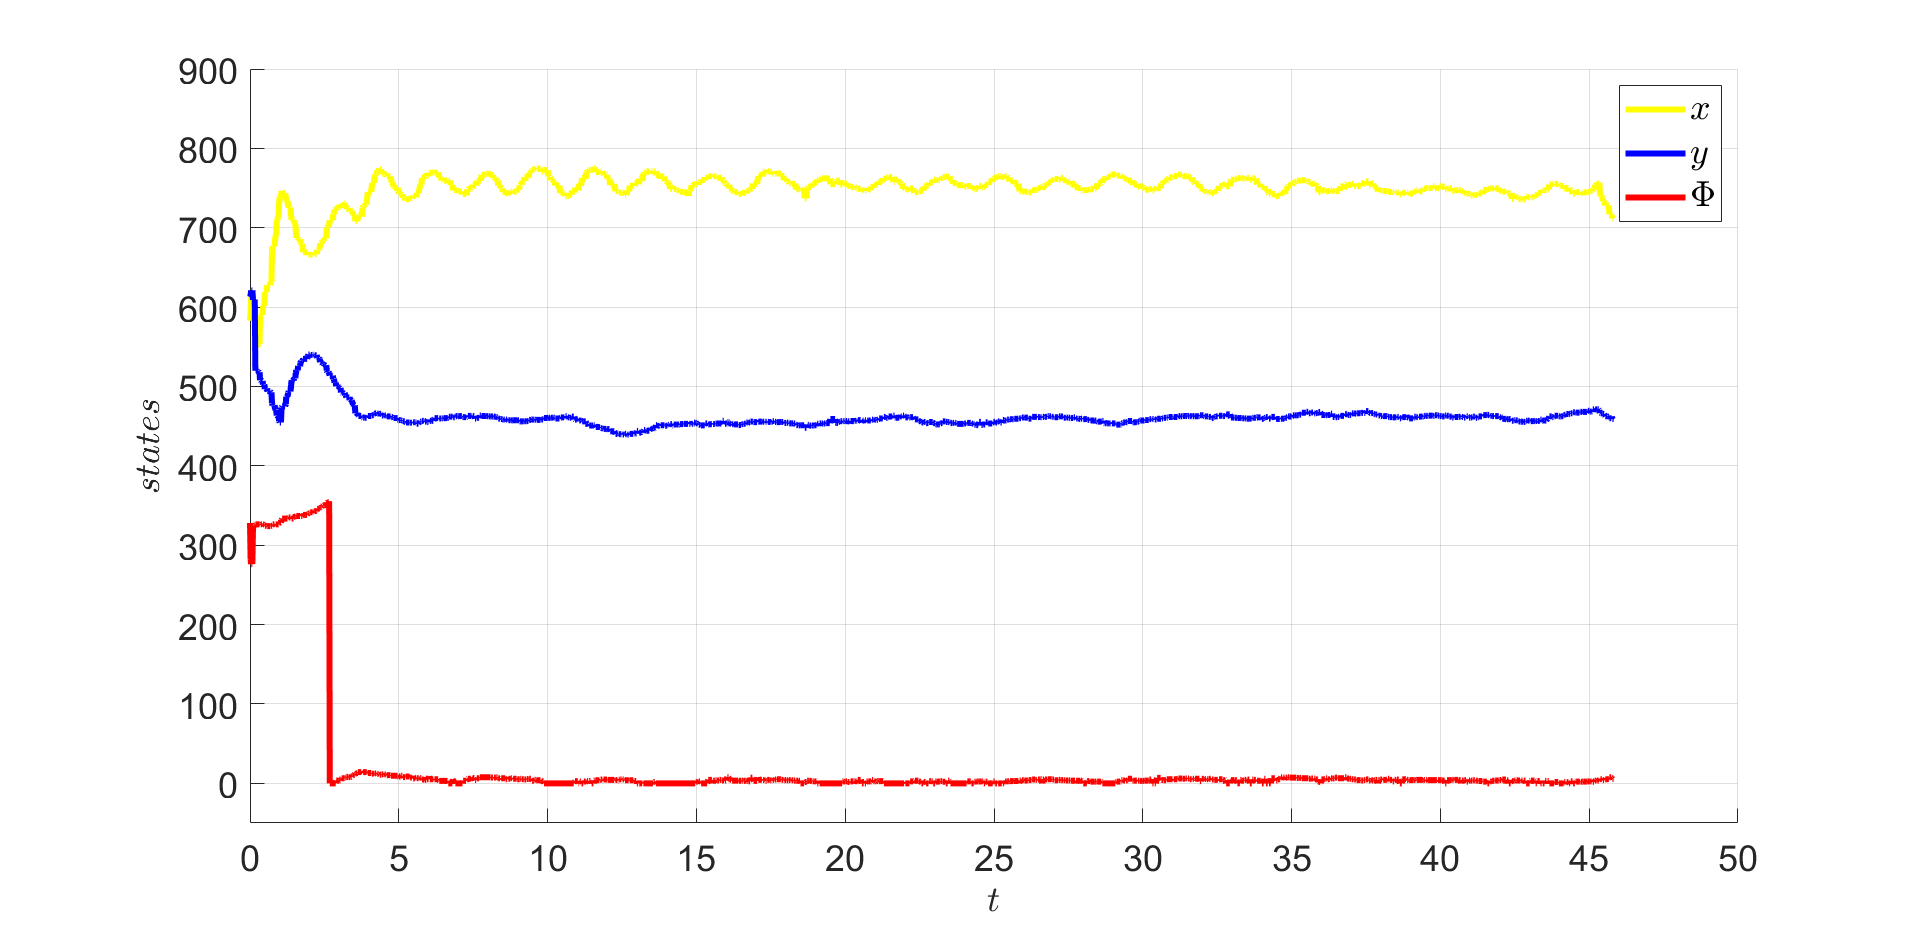
\includegraphics[width=\textwidth]{comp_x_1.png}
        \caption{эксперимент}
         \label{fig:comp_x_1.png}
     \end{subfigure}
     \hfill
     \begin{subfigure}{0.49\textwidth}
         \centering
         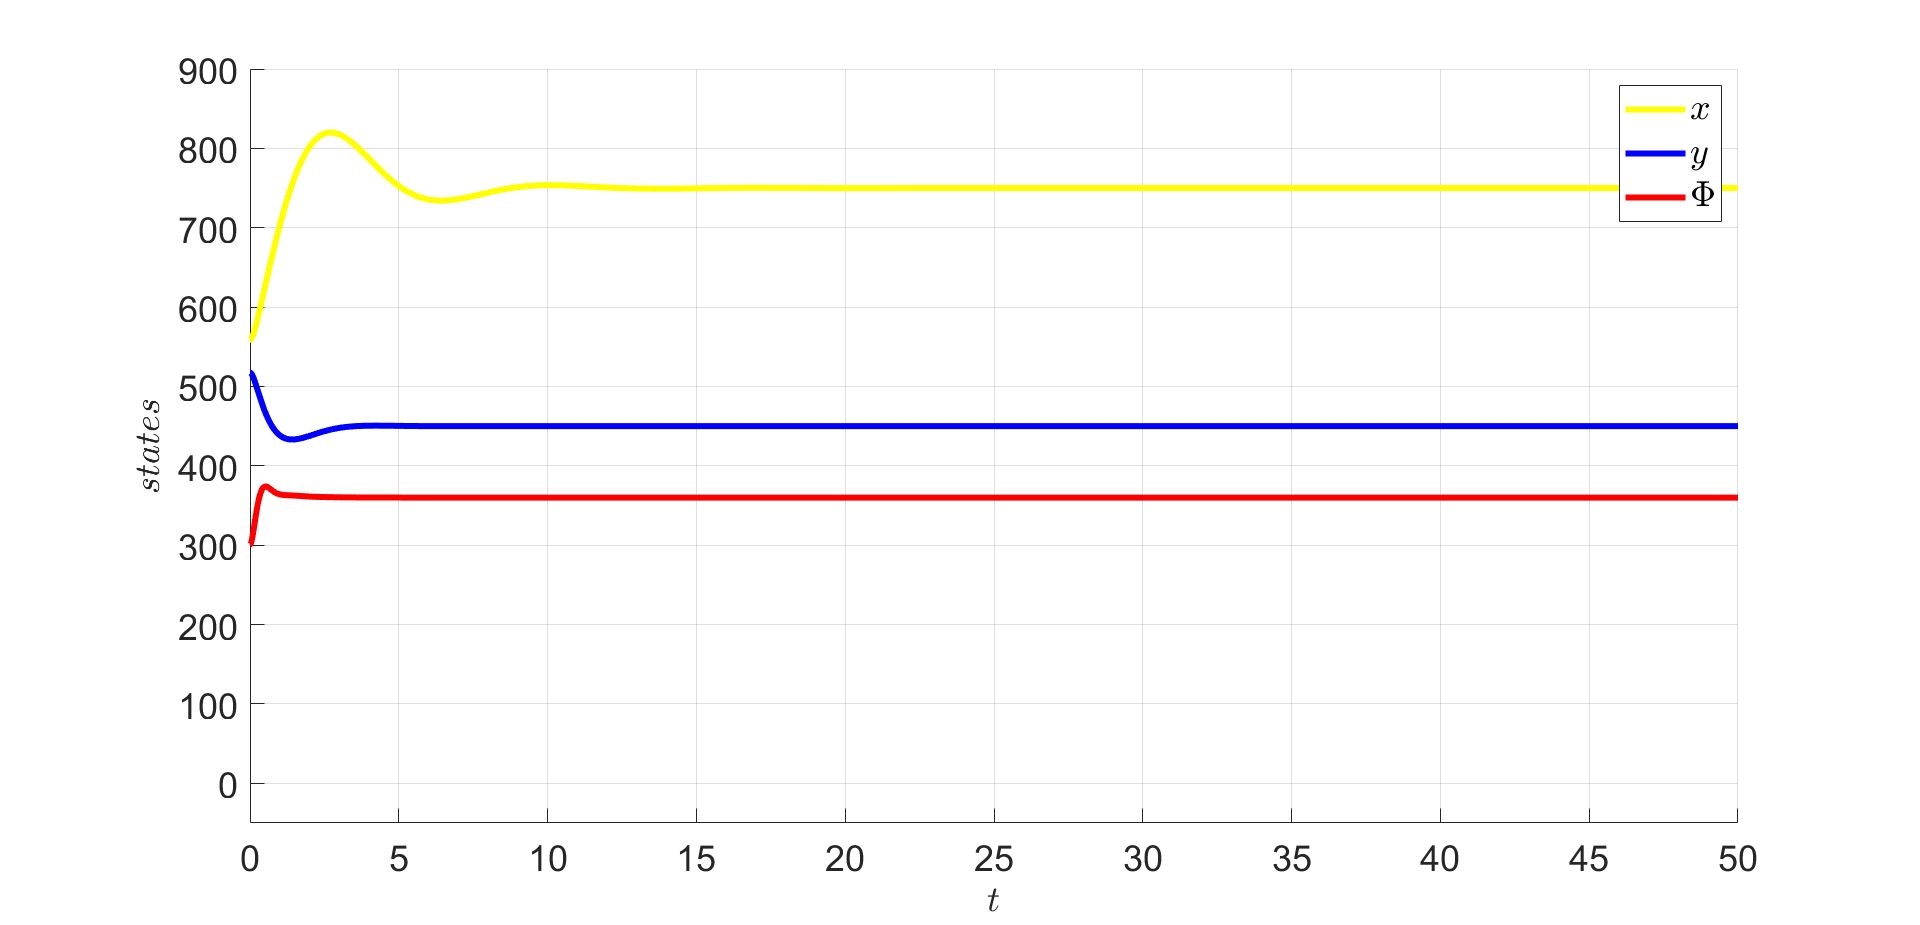
\includegraphics[width=\textwidth]{comp_x_modeling.png}
         \caption{моделирование}
         \label{fig:comp_x_modeling.png}
     \end{subfigure}
    \caption{Графики переходных процессов.}
    \label{fig:two graphs}
\end{figure}

\begin{figure}[H]
    \centering
    \begin{subfigure}{0.49\textwidth}
        \centering
        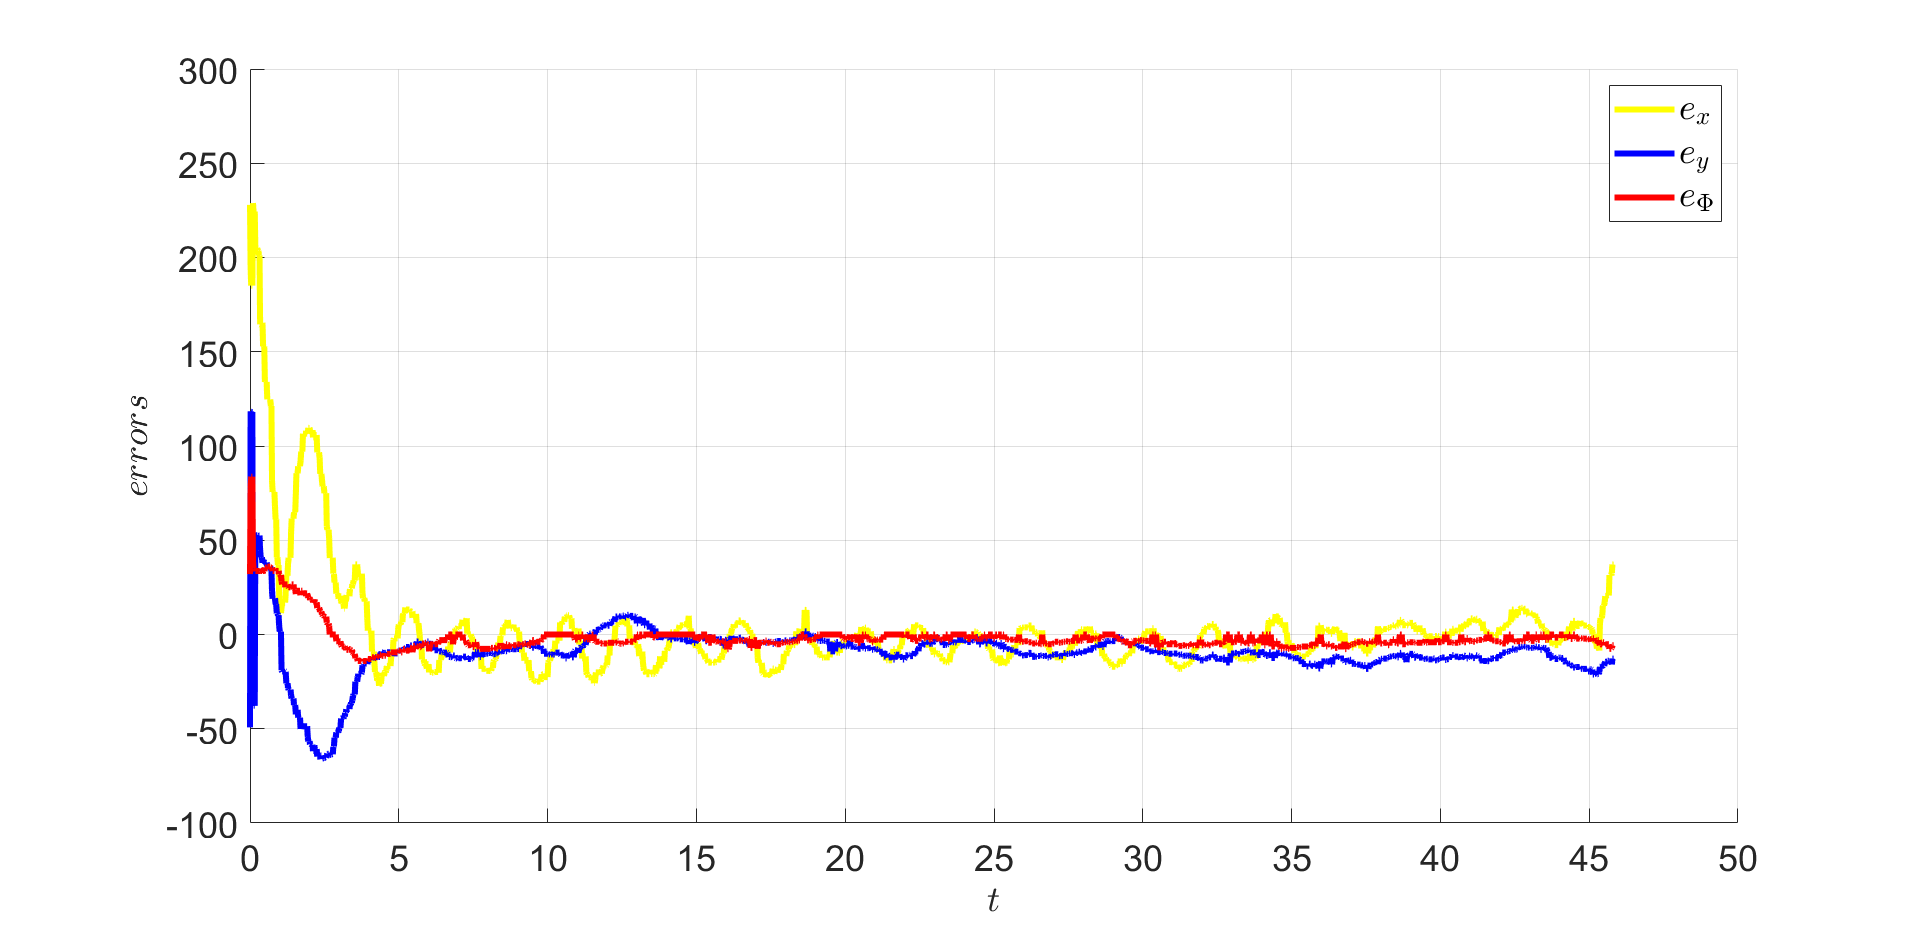
\includegraphics[width=\textwidth]{comp_e_1.png}
        \caption{эксперимент}
         \label{fig:comp_e_1.png}
     \end{subfigure}
     \hfill
     \begin{subfigure}{0.49\textwidth}
         \centering
         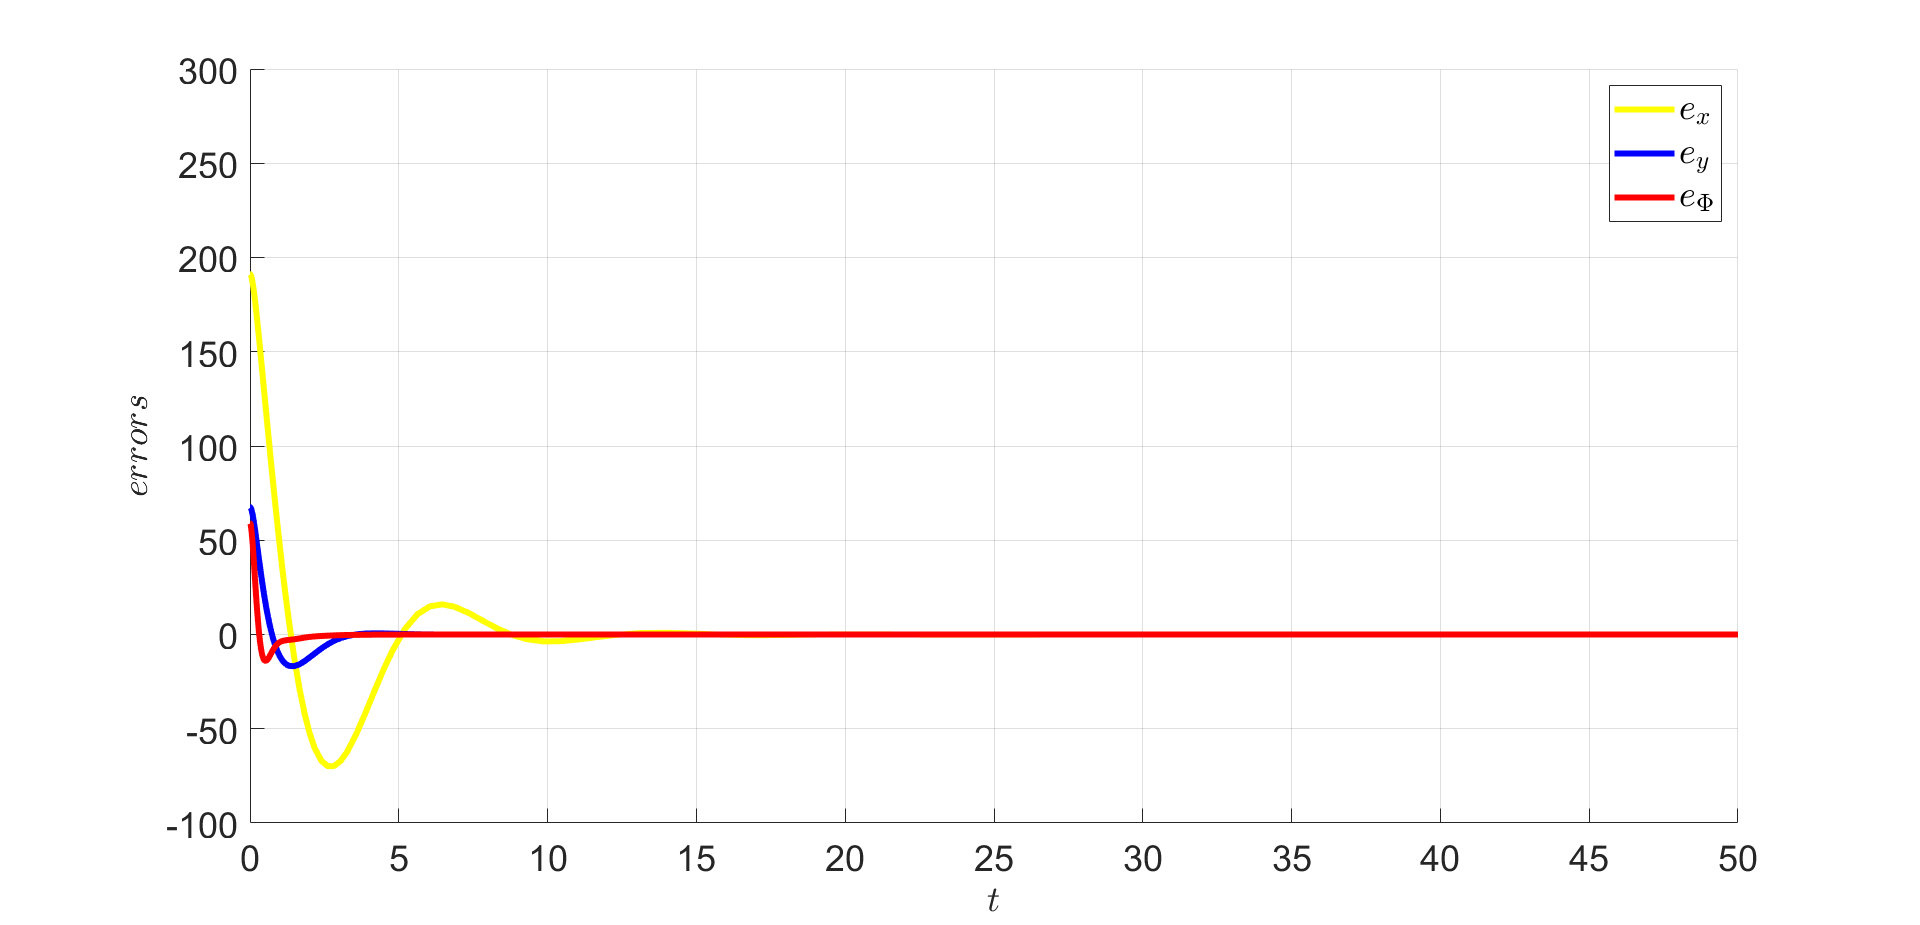
\includegraphics[width=\textwidth]{comp_e_modeling.png}
         \caption{моделирование}
         \label{fig:comp_e_modeling.png}
     \end{subfigure}
    \caption{Графики ошибок.}
    \label{fig:two graphs}
\end{figure}

Последовательный компенсатор смог за 5 секунд стабилизировать судно. Также, увеличилась точность регулятора в сравнении с обычным ПИД-регулятором. 

\section*{Управление на основе наблюдателя с высоким коэффициентом усиления}

Рассмотрим систему управления на основе наблюдателя с высоким коэффициентом усиления:
\[
\dot{\hat{\xi}} = A_0 \hat{\xi} + B_0 \tilde{y},
\]
где
\[
A_0 = \begin{bmatrix}
    -\kappa C_2 & I \\
    -\kappa^2 C_1 & 0 \\
\end{bmatrix}, \
B_0 = \begin{bmatrix}
    \kappa C_2 \\
    \kappa^2 C_1 \\
\end{bmatrix},
\]
где $I \in \mathbb{R}^{3 \times 3}$ - единичная матрица, $C_1, \ C_2 \in \mathbb{R}^{3 \times 3}$ -  положительно определенные матрицы такие, что
матрица
\[
\begin{bmatrix}
    -C_2 & I \\
    -C_1 & 0 \\
\end{bmatrix}
\]
гурвицева, $\kappa > 0$ - высокий коэффициент усиления.\\

Закон управления задается в виде
\[
\hat{u_s} = sat_L(K \hat{\xi}),
\]
где $sat_L(..)$ - гладкая функция насыщения с ограничениями $\pm L$, $\hat{\xi}$ - состояние наблюдателя, $K \in \mathbb{R}^{3 \times 6}$ - матрица настраиваемых коэффициентов.\\

\begin{figure}[H]
    \centering
    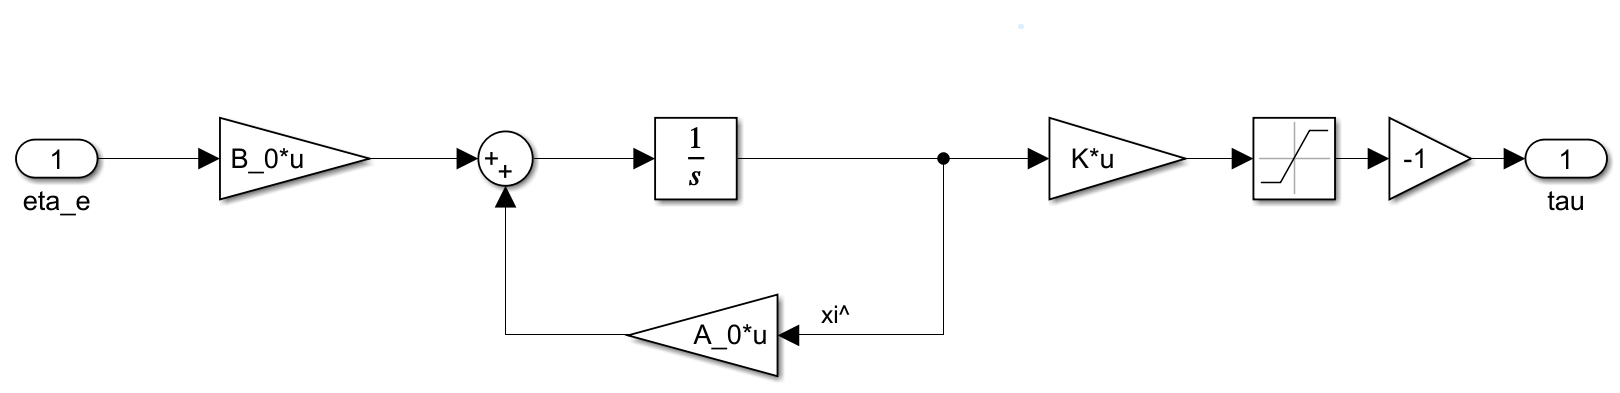
\includegraphics[width=\textwidth]{highgain_scheme.png}
    \caption{Блок-схема наблюдателя с высоким коэффициентом усиления.}
    \label{fig:highgain_scheme.png}
\end{figure}\\

Выбранные параметры модели:
\[
K = \begin{bmatrix}
    25 & 0 & 0 & 100 & 0 & 0 \\
    0 & 75 & 0 & 0 & 100 & 0 \\
    0 & 0 & 1000 & 0 & 0 & 100 \\
\end{bmatrix},
\]
\[
C_1 = \begin{bmatrix}
    1 & 0 & 0 \\
    0 & 2 & 0 \\
    0 & 0 & 3 \\
\end{bmatrix}, \ 
C_2 = \begin{bmatrix}
    4 & 0 & 0 \\
    0 & 5 & 0 \\
    0 & 0 & 6 \\
\end{bmatrix},
\]
\[
\kappa = 7, \ \lambda = 10.
\]

Эксперимент с high-gain наблюдателем был проведен при следующем начальном условии:
\[
y_{initial} = \begin{bmatrix}
    788 \\ 567 \\ 317
\end{bmatrix}.
\]
Референская точка:
\[
y_{goal} = \begin{bmatrix}
    750 \\ 450 \\ 0
\end{bmatrix}
\]
Приведем графики эксперимента и моделирования:
\begin{figure}[H]
    \centering
    \begin{subfigure}{0.49\textwidth}
        \centering
        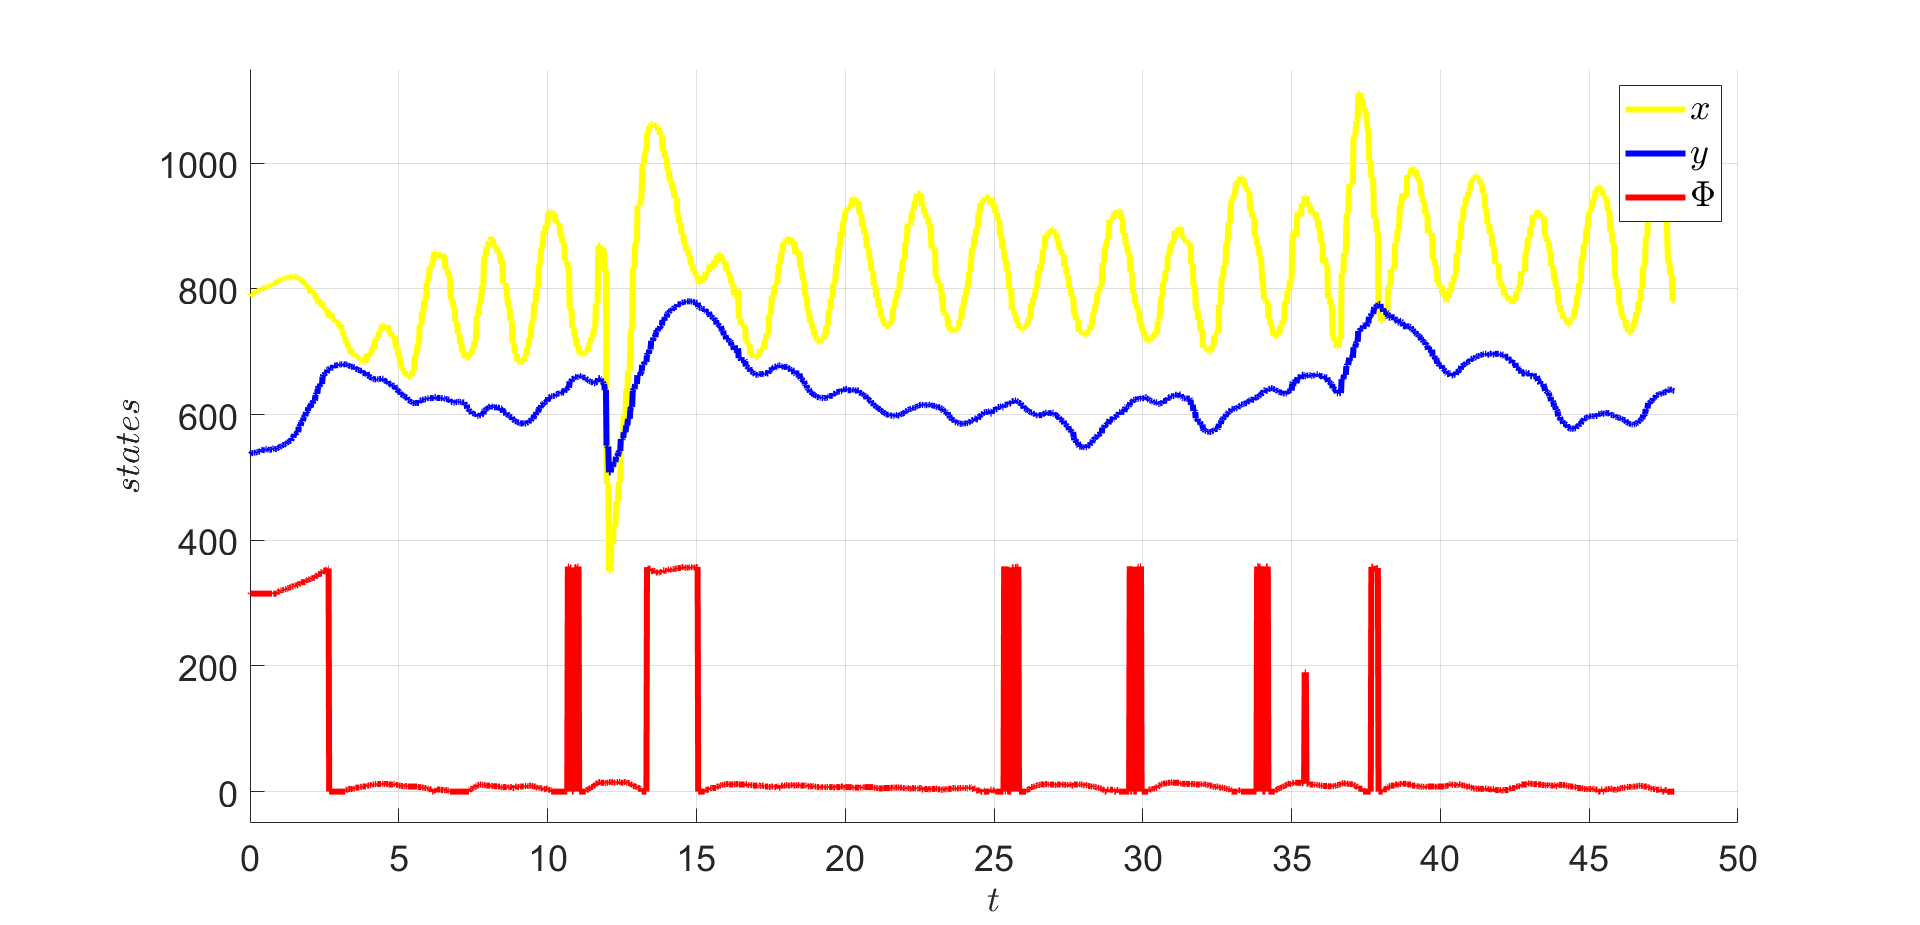
\includegraphics[width=\textwidth]{highgain_x.png}
        \caption{эксперимент}
         \label{fig:highgain_x.png}
     \end{subfigure}
     \hfill
     \begin{subfigure}{0.49\textwidth}
         \centering
         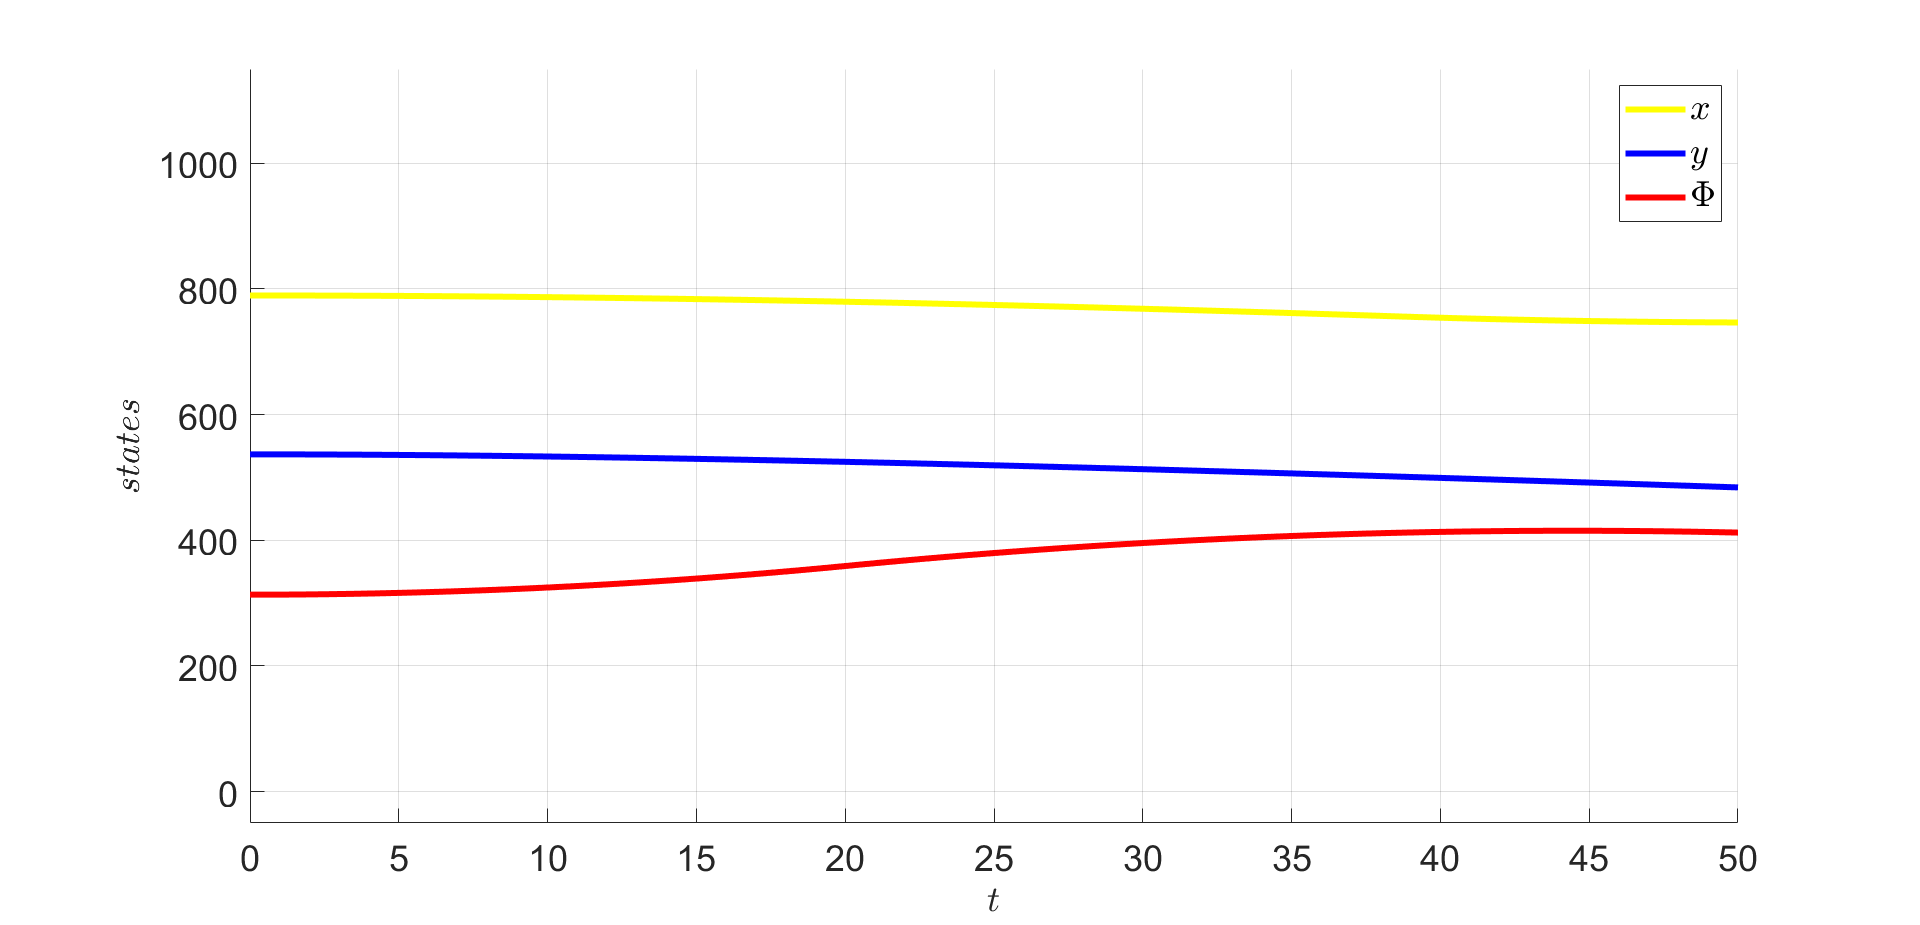
\includegraphics[width=\textwidth]{highgain_x_modeling.png}
         \caption{моделирование}
         \label{fig:highgain_x_modeling.png}
     \end{subfigure}
    \caption{Графики переходных процессов.}
    \label{fig:two graphs}
\end{figure}

\begin{figure}[H]
    \centering
    \begin{subfigure}{0.49\textwidth}
        \centering
        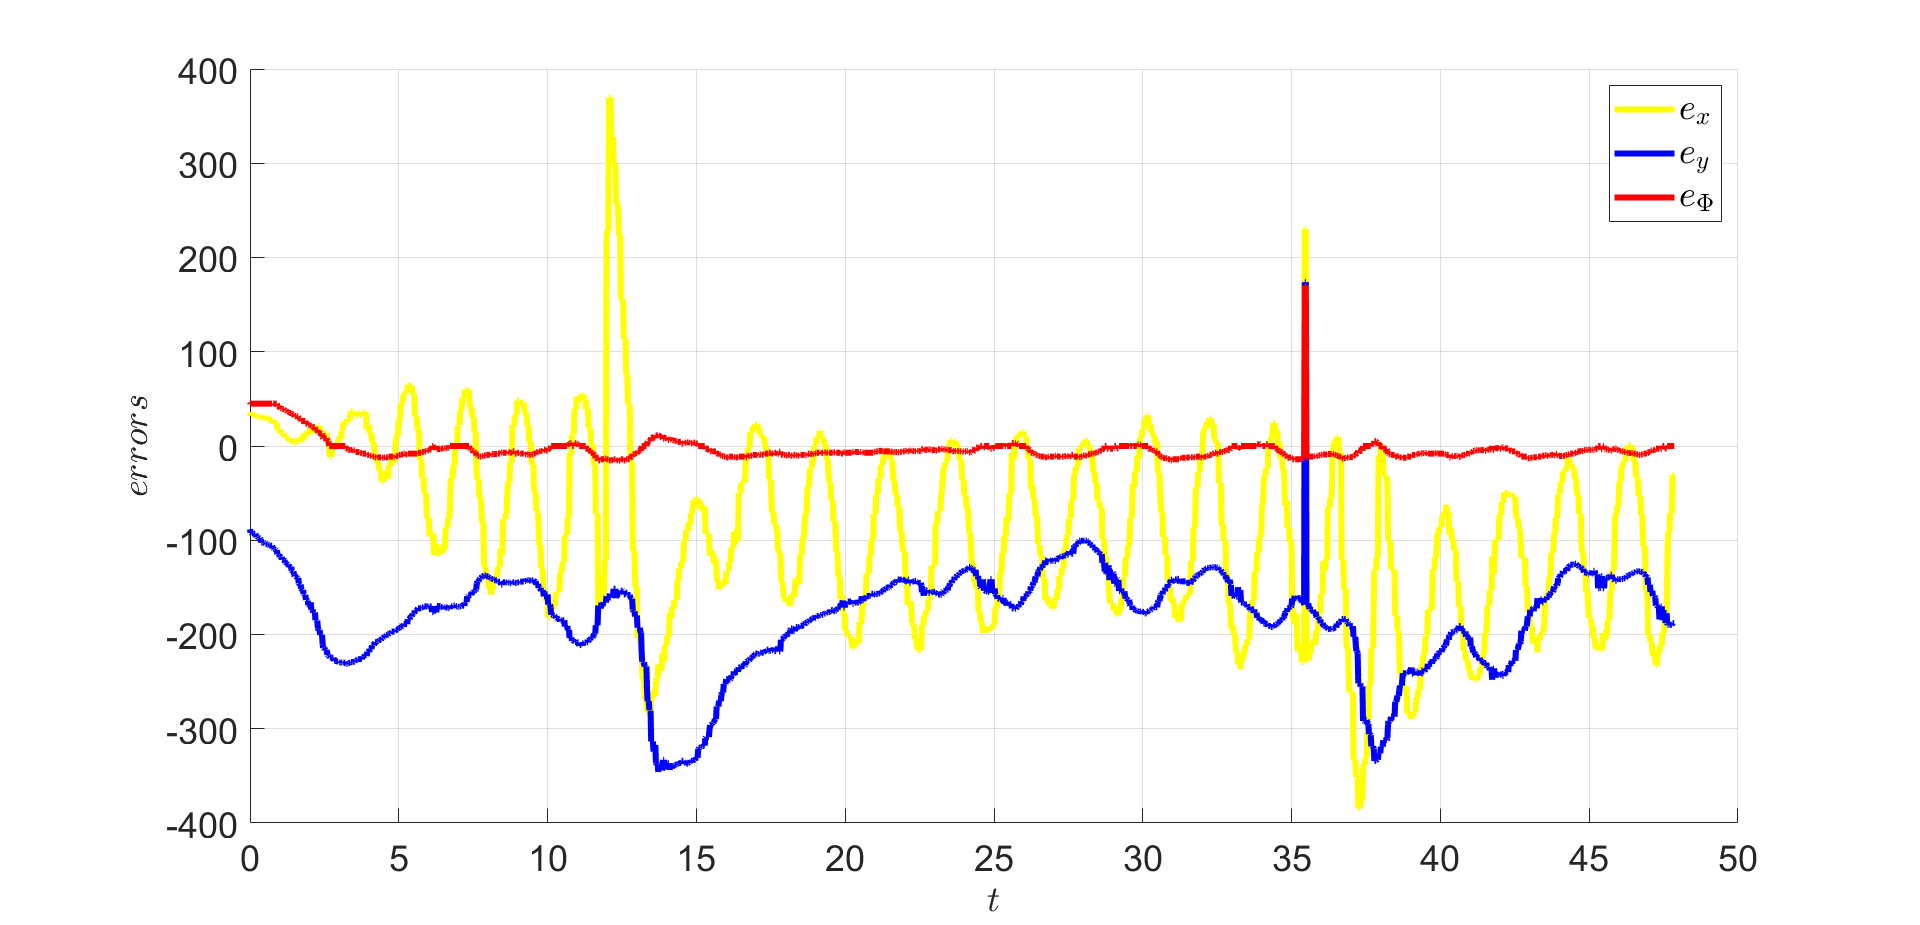
\includegraphics[width=\textwidth]{highgain_e.png}
        \caption{эксперимент}
         \label{fig:highgain_e.png}
     \end{subfigure}
     \hfill
     \begin{subfigure}{0.49\textwidth}
         \centering
         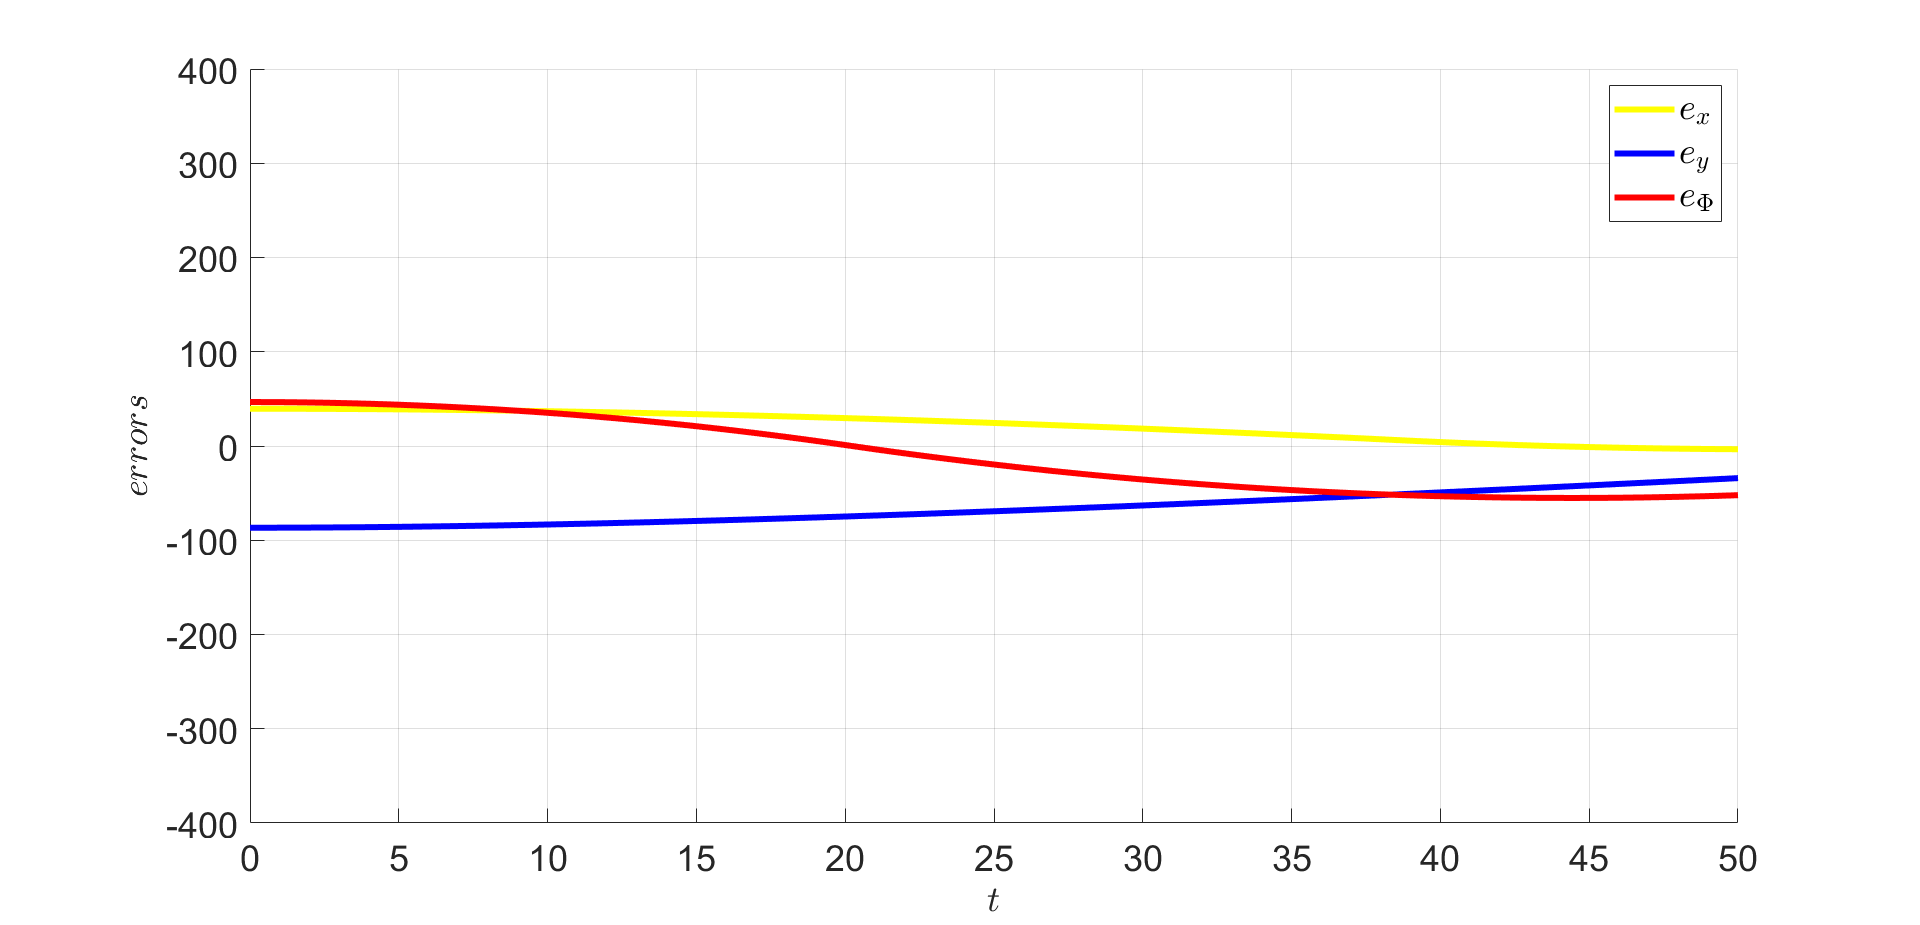
\includegraphics[width=\textwidth]{highgain_e_modeling.png}
         \caption{моделирование}
         \label{fig:highgain_e_modeling.png}
     \end{subfigure}
    \caption{Графики ошибок.}
    \label{fig:two graphs}
\end{figure}

Увеличим время моделирования до 500 секунд:
\begin{figure}[H]
    \centering
    \begin{subfigure}{0.49\textwidth}
        \centering
        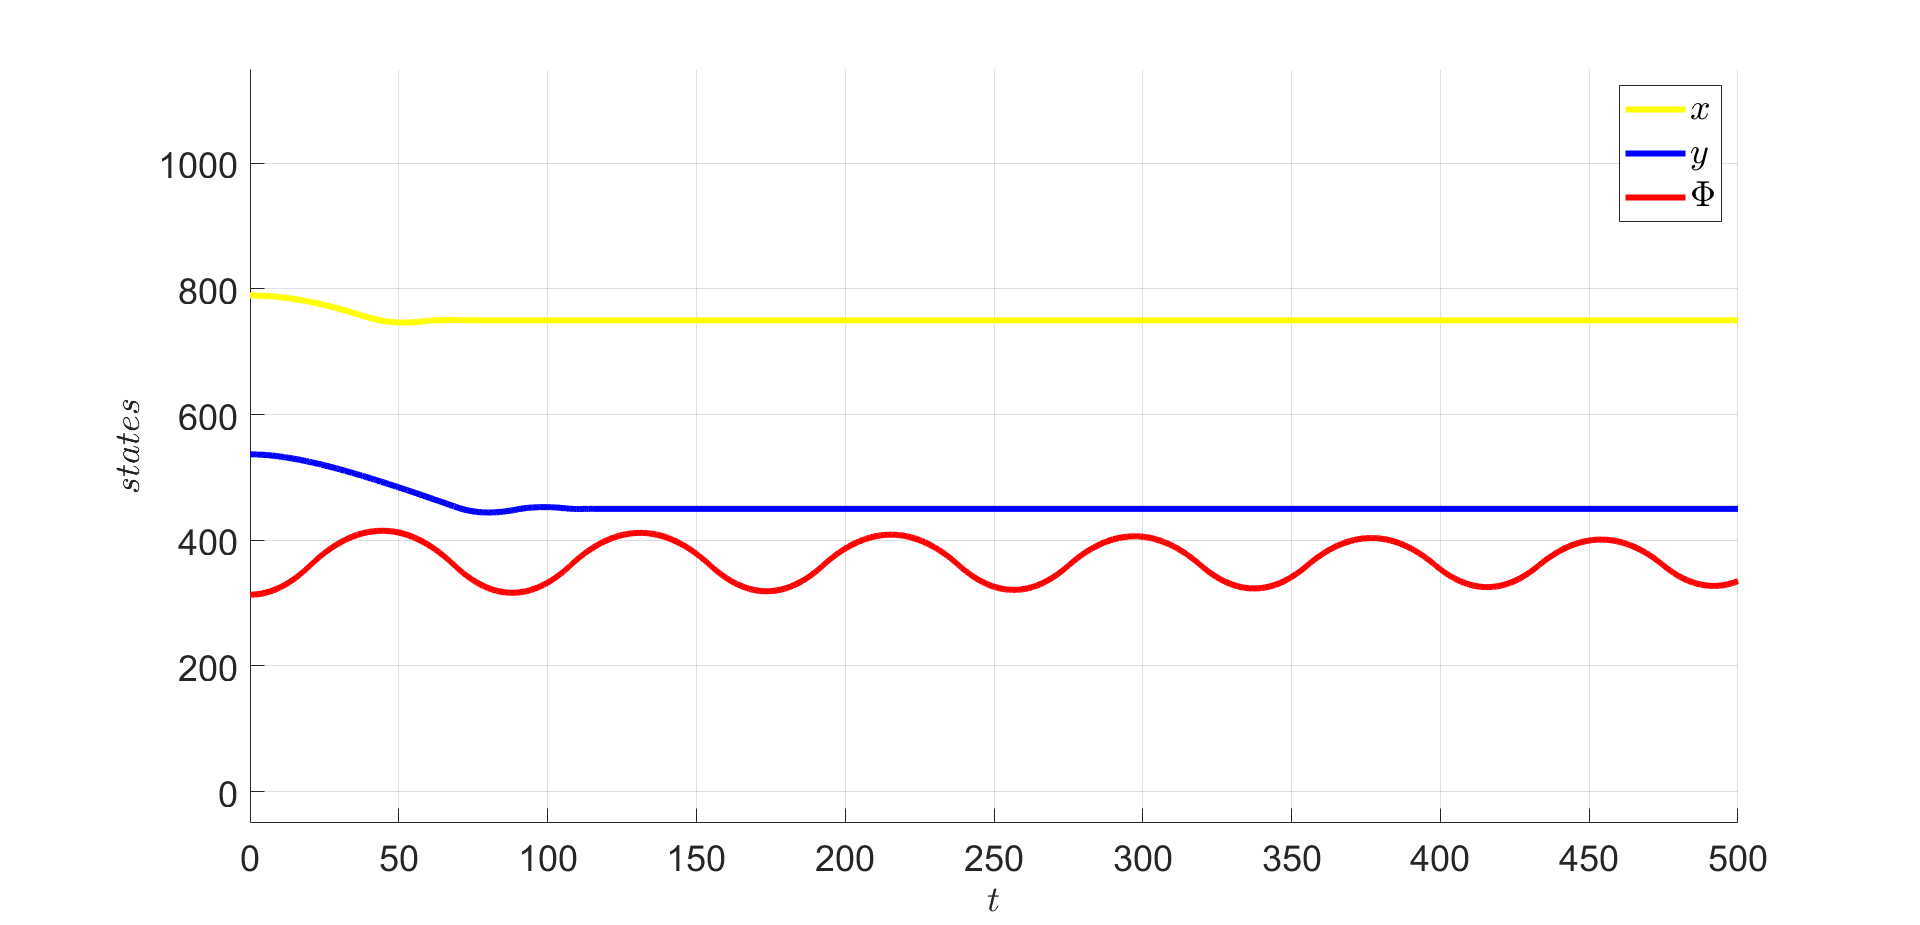
\includegraphics[width=\textwidth]{highgain_x_modeling_extended.png}
        \caption{состояния}
         \label{fig:highgain_x_modeling_extended.png}
     \end{subfigure}
     \hfill
     \begin{subfigure}{0.49\textwidth}
         \centering
         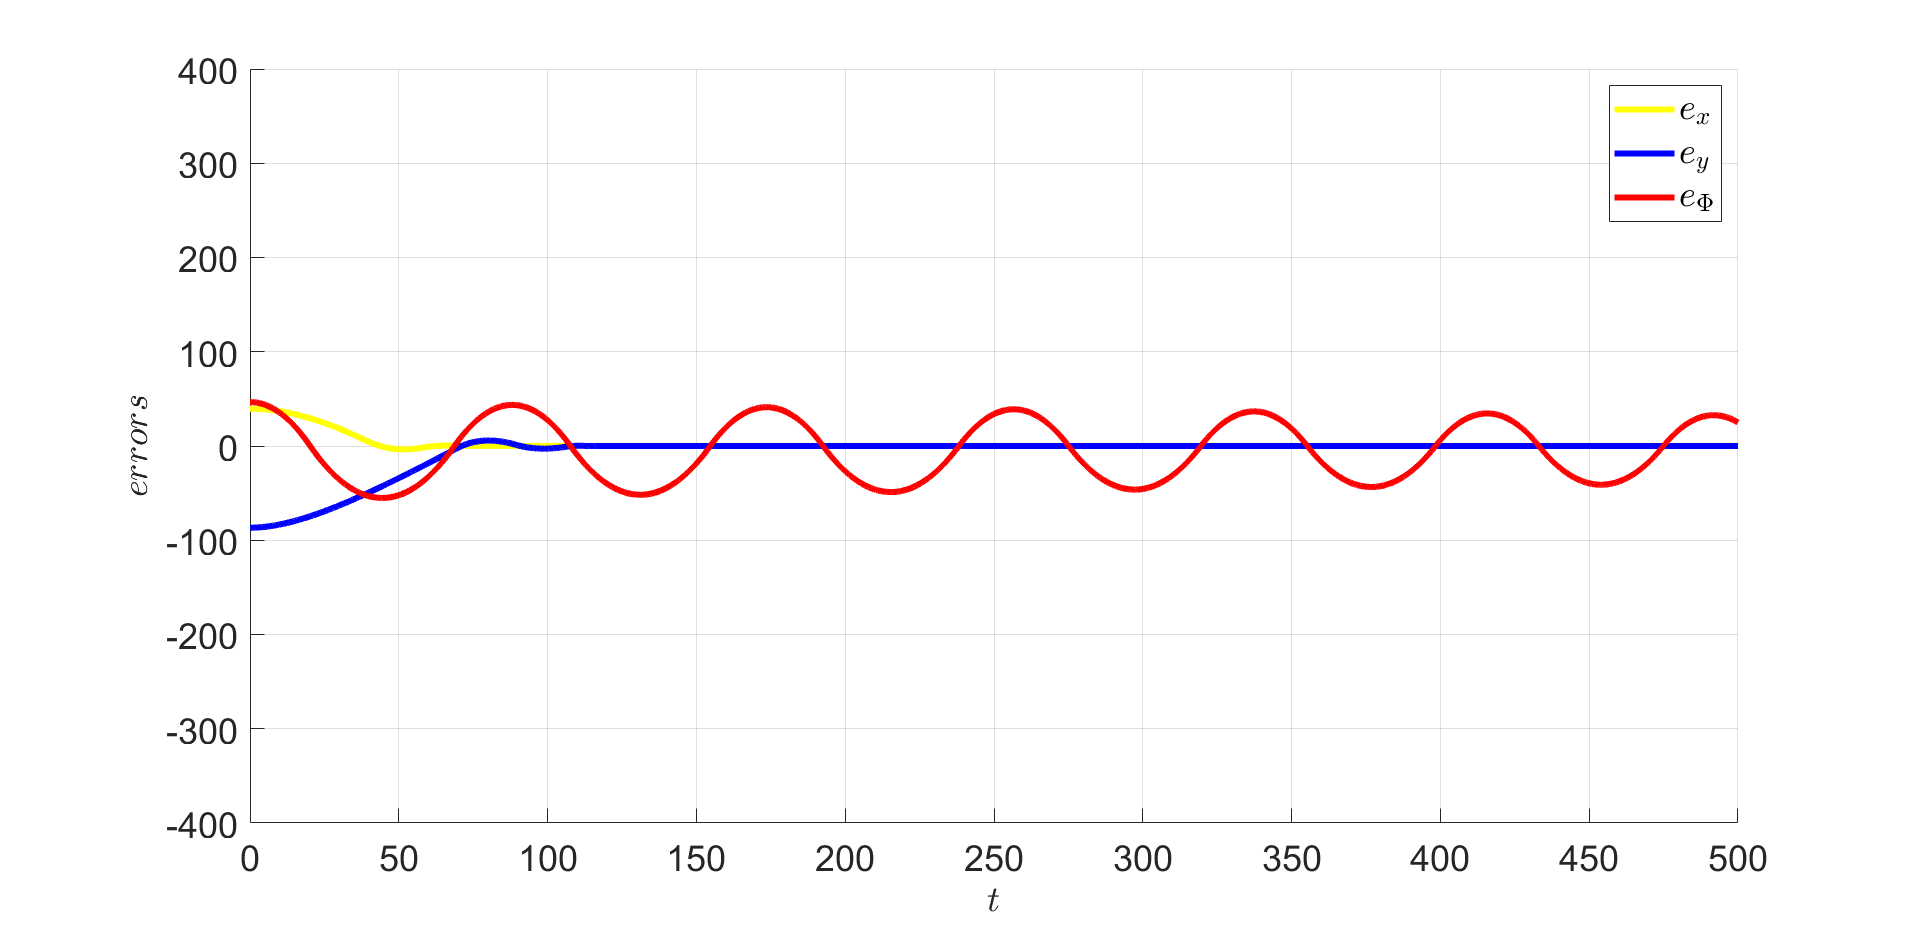
\includegraphics[width=\textwidth]{highgain_e_modeling_extended.png}
         \caption{ошибки}
         \label{fig:highgain_e_modeling_extended.png}
     \end{subfigure}
    \caption{Моделирование 500 секунд.}
    \label{fig:two graphs}
\end{figure}

Как видно по графикам, подобрать оптимальные значения параметров не удалось. Если в ходе моделирования данный регулятор смог стабилизировать положение за 40 секунд и по углу была колеблющаяся ошибка, то при эксперименте достичь сходимости ошибки не удалось совсем.\\

\section*{Выводы}
В данной лабораторной работе была рассмотрена задача стабилизации надводного судна (его линеаризованной модели) с помощью регуляторов трех типов (ПИД, последовательный компенсатор и наблюдатель с высоким коэффициентом усиления).\\
В начале требовалось реализовать данные регуляторы в Simulink, промоделировать поведение судна и подобрать оптимальные для моделирования коэффициенты.\\
Затем проводилась экспериментальная апробация алгоритмов. Результаты экспериментов для ПИД-регулятора и последовательного компенсатора были удовлетворительны, поведение системы было похоже на смоделированные графики переходных процессов и ошибок с точностью до внешних возмущений, колебаний воды, а также нелинейности системы. Эксперимент с high-gain наблюдателем не удался, так как подобранные в результате моделирования параметры не подошли для реальных опытов.\\
Наиболее эффективным методом управления в ходе данной работы стал последовательный компенсатор - у него более точная и быстрая стабилизация.
\end{document}